\chapter{Bangun Datar dan Bangun Ruang}\label{ch:g2:shapes}

Bangun datar hidup di atas kertas; bangun ruang memenuhi tanganmu.
Bab ini menggolongkan bangun datar dengan membilang sisi dan titik
sudut, menguji sudut siku-siku dengan pojok kertas yang dilipat, lalu
berkenalan dengan bangun ruang yang pertama --- yang sisinya adalah
bangun datar yang sudah kita kenal.

\section{Menggolongkan bangun datar}

\begin{definition}[Bersisi lurus dan bundar]\label{def:g2:shapes:sort}
Bangun yang tepinya hanya tersusun dari sisi lurus disebut
\emph{segi banyak}\index{segi banyak}: segitiga ($3$ sisi), segi empat ($4$ sisi:
persegi dan persegi panjang adalah segi empat), segi lima ($5$),
segi enam ($6$). Bangun yang tepinya melengkung, seperti lingkaran,
\emph{bukan} segi banyak.
\end{definition}

\begin{omfigure}
\begin{tikzpicture}[scale=0.62]
  \draw[thick, fill=omDef!12] (0,0) -- (1.8,0) -- (0.9,1.5) -- cycle;
  \node[below, font=\small] at (0.9,-0.35) {$3$ sisi};
  \begin{scope}[xshift=3.2cm]
  \draw[thick, fill=omThm!12] (0,0) rectangle (1.7,1.5);
  \node[below, font=\small] at (0.85,-0.35) {$4$ sisi};
  \end{scope}
  \begin{scope}[xshift=6.6cm]
  % segi lima diukur agar mengisi pita tinggi yang sama (0..1.5) dengan tetangganya
  \draw[thick, fill=omMeth!12] (0.95,0.67) +(90:0.83) -- +(162:0.83) --
    +(234:0.83) -- +(306:0.83) -- +(18:0.83) -- cycle;
  \node[below, font=\small] at (0.95,-0.35) {$5$ sisi};
  \end{scope}
  \begin{scope}[xshift=10.0cm]
  \draw[thick, fill=omProp!12] (0.75,0.75) circle (0.75);
  \node[below, font=\small] at (0.75,-0.35) {bundar};
  \end{scope}
\end{tikzpicture}

{\small Menggolongkan menurut banyaknya sisi. Banyaknya titik sudut
selalu sama dengan banyaknya sisi.}
\end{omfigure}

\begin{method}[Menguji sudut siku-siku]\label{met:g2:shapes:rightangle}
Lipatlah selembar kertas dua kali sampai terbentuk pojok yang tajam
--- pojok itu adalah sudut siku-siku. Tempelkan pada sudut sebuah
bangun:
\begin{enumerate}
  \item jika kedua sisi bangun itu berimpit tepat dengan pojok
        lipatan, sudutnya siku-siku;
  \item jika sudutnya lebih lebar atau lebih sempit, ia tidak siku-siku.
\end{enumerate}
Persegi dan persegi panjang punya empat sudut siku-siku.
\end{method}

\section{Menyalin di kertas berpetak}

\begin{method}[Menyalin sebuah gambar]\label{met:g2:shapes:copy}
Di kertas berpetak, salinlah gambar titik sudut demi titik sudut:
\begin{enumerate}
  \item pilihlah satu titik sudut lalu tandai di petak yang kosong;
  \item bilanglah petak sampai titik sudut berikutnya (``$3$ ke
        kanan, $2$ ke atas'') lalu tandai;
  \item hubungkan titik sudutnya berurutan; bandingkan dengan modelnya.
\end{enumerate}
\end{method}

\begin{omfigure}
\begin{tikzpicture}[scale=0.5]
  \draw[gray!40] (0,0) grid (5,4);
  \draw[thick, omDef] (1,1) -- (4,1) -- (4,3) -- (2,3) -- cycle;
  \begin{scope}[xshift=7cm]
  \draw[gray!40] (0,0) grid (5,4);
  \draw[thick, omThm] (1,1) -- (4,1) -- (4,3) -- (2,3) -- cycle;
  \node[font=\footnotesize, omThm, below] at (2.5,-0.15) {salinannya};
  \end{scope}
\end{tikzpicture}

{\small Sebuah gambar dan salinannya, dibuat dengan membilang petak
di antara titik sudutnya.}
\end{omfigure}

\section{Bangun ruang}

\begin{definition}[Bangun ruang yang pertama]\label{def:g2:shapes:solids}
Bangun ruang memakan tempat. Bidang datarnya disebut \emph{sisi}\index{sisi}:
\begin{itemize}
  \item \emph{kubus}\index{kubus}: $6$ sisi berbentuk persegi (sebuah dadu);
  \item \emph{balok}: $6$ sisi berbentuk persegi panjang (sebuah
        kotak sereal);
  \item \emph{tabung}\index{tabung}: dua sisi bundar dan satu sisi yang
        tergulung (sebuah kaleng);
  \item \emph{bola}: bundar sempurna, tanpa sisi datar.
\end{itemize}
Bangun ruang dan sisinya kembali pada \cref{ch:g5:solids}.
\end{definition}

\begin{omfigure}
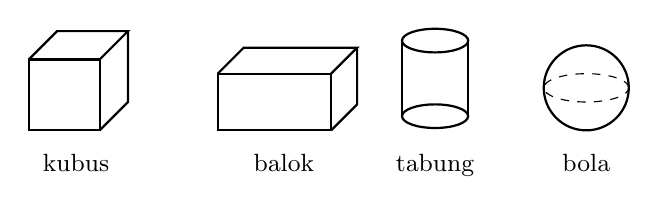
\begin{tikzpicture}[scale=0.6]
  \draw[thick] (0,0) rectangle (1.5,1.5);
  \draw[thick] (0,1.5) -- (0.6,2.1) -- (2.1,2.1) -- (1.5,1.5);
  \draw[thick] (2.1,2.1) -- (2.1,0.6) -- (1.5,0);
  \node[below, font=\small] at (1.0,-0.3) {kubus};
  \begin{scope}[xshift=4.0cm]
  \draw[thick] (0,0) rectangle (2.4,1.2);
  \draw[thick] (0,1.2) -- (0.55,1.75) -- (2.95,1.75) -- (2.4,1.2);
  \draw[thick] (2.95,1.75) -- (2.95,0.55) -- (2.4,0);
  \node[below, font=\small] at (1.4,-0.3) {balok};
  \end{scope}
  \begin{scope}[xshift=8.6cm]
  \draw[thick] (0,0.3) ellipse (0.7 and 0.25);
  \draw[thick] (-0.7,0.3) -- (-0.7,1.9);
  \draw[thick] (0.7,0.3) -- (0.7,1.9);
  \draw[thick] (0,1.9) ellipse (0.7 and 0.25);
  \node[below, font=\small] at (0,-0.3) {tabung};
  \end{scope}
  \begin{scope}[xshift=11.8cm]
  \draw[thick] (0,0.9) circle (0.9);
  \draw[dashed] (0,0.9) ellipse (0.9 and 0.3);
  \node[below, font=\small] at (0,-0.3) {bola};
  \end{scope}
\end{tikzpicture}

{\small Bangun ruang yang pertama. Rabalah sebuah \omterm{def:g2:shapes:solids}{kubus} dengan jari:
kamu merasakan $6$ sisi datar dan rusuk yang tajam; bola tidak punya keduanya.}
\end{omfigure}

\section{Latihan}

\begin{exercise}[$\star$]\label{exo:g2:shapes:1}
Untuk masing-masing, bilanglah sisi dan titik sudutnya lalu namailah:
bangun dengan $5$ sisi; bangun dengan $3$ titik sudut; bangun bundar.
\end{exercise}

\begin{exercise}[$\star$]\label{exo:g2:shapes:2}
Golongkan menjadi ``\omterm{def:g2:shapes:sort}{segi banyak}'' atau ``bukan \omterm{def:g2:shapes:sort}{segi banyak}'':
persegi; lingkaran; segitiga; segi enam.
\end{exercise}

\begin{exercise}[$\star$]\label{exo:g2:shapes:3}
Buatlah penguji sudut siku-siku dengan melipat kertas. Carilah tiga
sudut siku-siku di dalam ruangan, dan satu sudut yang tidak siku-siku.
\end{exercise}

\begin{exercise}[$\star$]\label{exo:g2:shapes:4}
Berapa sudut siku-siku pada persegi? Pada persegi panjang? Paling
banyak berapa pada segitiga? (Cobalah menggambar segitiga dengan dua.)
\end{exercise}

\begin{exercise}[$\star$]\label{exo:g2:shapes:5}
Di kertas berpetak, salinlah persegi panjang selebar $4$ petak dan
setinggi $2$ petak, lalu segitiga dengan alas $3$ petak.
\end{exercise}

\begin{exercise}[$\star$]\label{exo:g2:shapes:6}
Sebutkan bangun ruangnya: sebuah dadu; sekaleng sup; sebuah bola sepak; sebuah kotak sepatu.
\end{exercise}

\begin{exercise}[$\star$]\label{exo:g2:shapes:7}
Berapa sisi sebuah \omterm{def:g2:shapes:solids}{kubus}? Setiap sisinya berbentuk apa? Berapa sisi
sebuah balok?
\end{exercise}

\begin{exercise}[$\star$]\label{exo:g2:shapes:8}
Bangun ruang mana yang dapat menggelinding: \omterm{def:g2:shapes:solids}{kubus}, balok, bola, atau
\omterm{def:g2:shapes:solids}{tabung}? Mengapa?
\end{exercise}

\begin{exercise}[$\star$]\label{exo:g2:shapes:9}
Sebuah bangun punya $6$ sisi. Apa namanya? Berapa titik sudutnya?
\end{exercise}

\begin{exercise}[$\star\star$]\label{exo:g2:shapes:10}
Di kertas berpetak, gambarlah sebuah rumah: persegi untuk dindingnya
($4 \times 4$) dengan atap segitiga di atasnya. Berapa sisi dan titik
sudut pada seluruh tepi rumah itu?

\end{exercise}
